\documentclass[sigplan,nonacm]{acmart}
\settopmatter{printfolios=true}
\usepackage{graphicx} % Required for inserting images
\graphicspath{ {./images/} } %images subfolder
\usepackage[normalem]{ulem}

\title{Related Works}
\author{Mark Madler}
\begin{document}
\maketitle
%All are related to some degree -- so they are organized as follows:

%                       REPLICATED KVS
%------------------------------------------------------------------------------------

\section{KVS over RDMA}

    \subsection{Kite: efficient and available release consistency for the datacenter}
    This is the real entry paper. This is a replicated KVS over RDMA with a 
    "Linearizable variant of" \textbf{Release Consistency}. Some mention of Release Consistency
    as a "one sided barrier." Compares against Zookeeper and Derecho. Uses some 
    monotonically increasing clocks to track versions.\cite{Gavrielatos-PPoPP-2020} 

    \subsection{FaRM: Fast Remote Memory}
    Super similar to the entry paper in that is is a KVS for RDMA, but this one is I beleive either disaggregated or not. 
    Farm could really be classified as a KVS or even a protocol. This design always replicates state info. 
    Provides \textbf{strict serializability}, so Transaction based consistency.
    So FaRM provides lock-free reads. The authors mention
    a "shared address space." \cite{Dragojevic-NSDI-2014}

    \subsection{FaRMv2: Fast General Distributed Transactions with Opacity}
    Just like FaRM but with opacity. Also providing \textbf{strict serializability}.
    Idk if this paper is really something to look at or not (TODO)\cite{Shamis-SIGMOD-2019}

    \subsection{HERD: Using RDMA efficiently for key-value services}
    Herd. Fast because it uses a weird combination of UD and message things.
    This combination is essentiall UC (unreliable connection) requests places 
    as writes to the server, then serviced by a server polling thread. The server replies over 
    UD (unreliable datagram) (this is a 2-sided send). One of the main ideas 
    of this paper is that writes can be faster than reads because there is 
    (at least with unreliable connection) no need for the destination to respond. 
    In the future it might be wise to refer back to this paper for info about the performance 
    metrics from RDMA verbs.\cite {Kalia-SIGCOMM-2014}

    \subsection{Sherman: A Write-Optimized Distributed B+Tree Index on Disaggregated Memory} %% start here %%
    This system is disaggregated. Node-granularity. "consistent". Optimizations are established
    to target mainly chained atomic operations and write-amplification. \cite{Wang-SIGMOD-2022}

    \subsection{Using One-Sided RDMA Reads to Build a Fast, CPU-Efficient Key-Value Store (Pilaf) }
    Linearizable data store.  Self-correcting. Note that this paper has a great 
    analysis of IPoIB as well as RDMA vs verbs latency and thrup. \cite{Mitchell-ATC-2013}

    %%  NEWLY ADDED  %%
    \subsection{Scythe: A Low-Latency RDMA-enabled Distributed Transaction System for Disaggregate Memory }
    KVS again. Seels to optimize concurrency control, timestamping, bandwidth. Uses Timestamp Oracle (TSO)
    hot-aware concurrecy control. Allows RPC. \cite{Lu-ACMtrans-2024}

    \subsection{HCL: Distributing Parallel Data Structures in Extreme Scales}
    Strictly serializabile KVS. HCL stands for Hermes Containder Library. \cite{Devarajan-CLUSTER-2020}

    \subsection{BCL: A Cross-Platform Distributed Data Structures Library}
    Confusingly uses either MPI, OpenSHMEM, GASNET-EX, and UPC++ as backends. Must be slow. \cite{Brock-ICPP-2019}
    
    \subsection{Rolex}
    I don't think this one really works. Uses learned indexes. splits compute and memory. \cite{Li-FAST-2023}

    \subsection{Exploiting Hybrid Index Scheme for RDMA-based Key-Value Stores*** (Hstore)}
    Seeks to solve issue of range-lookups. Compares against Sherman and Clover( LOOK INTO CLOVER). 
    This does indeed outperform sherman on YCSB. Maybe problematic for LOCO. claims 54\% improvement 
    over sherman.\cite{Han-SYSTOR-2023}

    \subsection{Disaggregating Persistent Memory and Controlling Them Remotely: An Exploration of Passive Disaggregated Key-Value Stores}
    "Clover". Workes on Persistent memory. A bit older, not worth comparing against unless looking into PM. also maybe faster 
    than Sherman but definitely not the fastest.\cite{Tsai-USENIX-2020}

    \subsection{AStore: Uniformed Adaptive Learned Index and Cache for RDMA-Enabled Key-Value Store}
    Supposedly outperforms \textbf{Sherman} by A LOT. ALso compares against "xstore" "Rolex" and "hybrid (not to be confused
    with the above hybrid index scheme which also independetly claims to be faster than Sherman)". 
    The results also suggest that Rolex outperforms \textbf{Sherman}. claims up to 91\% improvement over \textbf{Sherman}\cite{Qiao-IEEEtrans-2024}

    \subsection{Maintaining Cache Consistency in RDMA-based Distributed Key-Value storage System}
    note really worth considering it seems. This is indeed a KVS but only seems to compare against scale store. \cite{Hou-DSIT-2024}

    \subsection{FastStore: A High-Performance RDMA-Enabled Distributed Key-Value Store with Persistent Memory}
    not really worth considering. Again PM. COmpares against Clover and Sherman. Also is faster than Sherman with lower latency 
    as well as higher throughput. \cite{Xiong-ICDCS-2023}

    \subsection{LoLKV: The Logless, Linearizable, RDMA-based Key-Value Storage System}
    Weirdly does not compare against state of the art really. All of the comparisons are against older consensus protocols.
    LoLKV is worth looking at, but sincethere are no comparisons against Sherman I am more worried about the other papers 
    that do. It seems like this paper is more concerned about the consensus protocols. \cite{Alquraan-NSDI-2024}
%                       DSM OVER RDMA
%-----------------------------------------------------------------------------------
\section {DSM systems}

    \subsection{Scaling out NUMA-Aware Applications with RDMA-Based Distributed Shared Memory: MAGI}
    Page-based DSM. \textbf{Sequentially consistent} with the option of overriding in some cases. They use 
    smaller page sizes to try and over come page-based problems like write-amplification. They implement 
    strategies from traditional shared memory systems to enahnce their performance. They use specualtive 
    page faults to fetch pages before they are needed. Since the TLB is used extensively to maintain 
    a coherence within a node in terms of page visibility, there is a large overhead in the form of interrupts.
    The authors decided to batch these interrupts for improved performance. Unfortunately they have weak results
    which slow slight improvements over a "baseline" but do not compare against anything else. The baseline seems to be 
    their DSM without the speculation and batching.\cite{Hong-JCST-2019}

    \subsection{Efficient Distributed Memory Management with RDMA and Caching (GAM) }
    cache-line granularity DSM. Directory based, \textbf{Partial Store Order}. \textbf{PGAS addressing model}. 
    Use the directory to track the cache state at each node (DRMA cache). Attempsts to implement LRU 
    caching.  \cite{Cai-VLDB-2018}

    \subsection{Distributed Shared Object Memory}
    object based granularity, release consistency... too old for RDMA\cite{Guedes-WWOSIII-1993} %idk if worth reading

    \subsection{Gengar: An RDMA-based Distributed Hybrid Memory Pool}
    This is object based dsm over rdma but with non-volatile memory as well using Intel Optane. Seems to 
    also use this lease assignment idea like in \cite{Endo-IPDRM-2020} but is not page based. Uses a client / 
    server model where the servers provide DRAM and NVM to clients. The distributed DRAM is like a write-through 
    cache where the writes go through to Persistent memory. For some reason they provide longer leases 
    for hot objects (seems like this would increase worst case latency). Good results. \cite{Duan-ICDCS-2021}

    \subsection{TreadMarks: shared memory computing on networks of workstations}
    Was implemented over IP, lazy release consistency. Uses diffs to allow for multiple-writers. 
    Uses the page-size granularity, but diffs make this a little different. Also optimized for multiple threads
    on a local machine accessing the same page. \cite{Amza-Usenix-1994}

    \subsection{LITE Kernel RDMA Support for Datacenter Applications}
    This is page based DSM using the kernel. Has some care for permissions and security which is nice. 
    Claims to have more scalable thorughput than standard verbs. they run a DSM over their implementation.
    So this is not exactly a DSM but rather a way of using RDMA generally. \cite{Tsai-SOSP-2017}

    \subsection{MENPS: A Decentralized Distributed Shared Memory Exploiting RDMA} %% deep read this %%
        \begin{itemize}
            \item Page based DSM
            \item Special Diff merging and page sharing
            \item Combine write notices and logical leases (what is that?)\cite{Endo-IPDRM-2020}
        \end{itemize}

    \subsection{Argo DSM} 
    Page-based DSM. The authors propose a coherence trick where nodes will self-invalidate 
    or self-downgrade to avoid coherence traffic. They implement a message-free protocol (one sided verbs). 
    Built on top of MPI. Aim to resuce cost of directory based coherence. One of the main ideas is that 
    a node may read any data block as long as it will invalidate that data at the next synchronization point. \cite{Kaxiras-HPDC-2015}

    \subsection {GiantVM: A Novel Distributed Hypervisor for Resource Aggregation with DSM-aware Optimizations}
    Page-based DSM again but also works over TCP and RDMA. Basically its a distributed virtual CPU. It seems like 
    it is just a global address space that is known to the Hypervisor.\cite{Jia-ACO-2022}

    \subsection{Scalable RDMA performance in PGAS languages}
    This paper is for PGAS languages. Has an address hash table similar to LOCO for remote lookups. Written in 
    collaboration with IBM and details  the IBM XLUPC compiler + runtime. Some caching for performance. A little old of a paper
    so things like UPC++ were not around yet.\cite{Farreras-IPDPS-2009}

    \subsection {misc RDMA coherence papers}

    \subsection{Misc PGAS languages probably}
%-----------------------------------------------------------------------------------------
%                       PROTOCOLS OVER RDMA FOR CONSISTENCY
%----------------------------------------------------------------------------------------
\section{Protocols over RDMA for Consistency}

    \subsection{Notes on PGAS and "protocols"}
    It seems like there are not agreed upon semantics on what is a protocol. PGAS is a 
    memory model. For myself and posterity, PGAS is a memory model where the address space is logicaly partitioned across nodes.
    This means that there can be some reasoning about locality likely from virtual memory addresses.

    Some notes on MPI. MPI is a programming model which supports multiple communication backends. MPI 
    can run over IP, RDMA, etc. 

    \subsection {Odyssey: The Impact of Modern Hardware on Strongly-Consistent Replication Protocols}
    This paper is a summary of protocols used for RDMA communication. These protocols were used to 
    enforce consistency and were tested with a series of KVSs. This paper is related to Kite (same authors) 
    and Kite is one of the KVSs tested.\cite{Gavrielatos-EuroSys-2021}

    \subsection {Hermes: A Fast, Fault-Tolerant and Linearizable Replication Protocol}
    This paper \cite{Katsarakis-ASPLOS-2020} is one of the Protocols tested by the above paper Odyssey \cite{Gavrielatos-EuroSys-2021}. This 
    protocol guarantees linearizablity and is designed to work on replicated store systems.

    \subsection {Hamband: RDMA Replicated Data Types}
    This paper \cite{Houshmand-PLDI-2022} designed new RDMA data types that are replicated across nodes. This paper 
    is sort of a protocol paper as it implements this protocol to keep replicated data through either relaxed or 'strong consistency'.

    \subsection{Evaluation of RDMA opportunities in an Object-Oriented DSM}
    Interesting result is that it proves that invalidation protocols are better suited 
    for distributed systems. \cite{Veldema-LCPC-2007}
%----------------------------------------------------------------------------------------
%                       AWESOME TABLE
%----------------------------------------------------------------------------------------
\section{table i found}
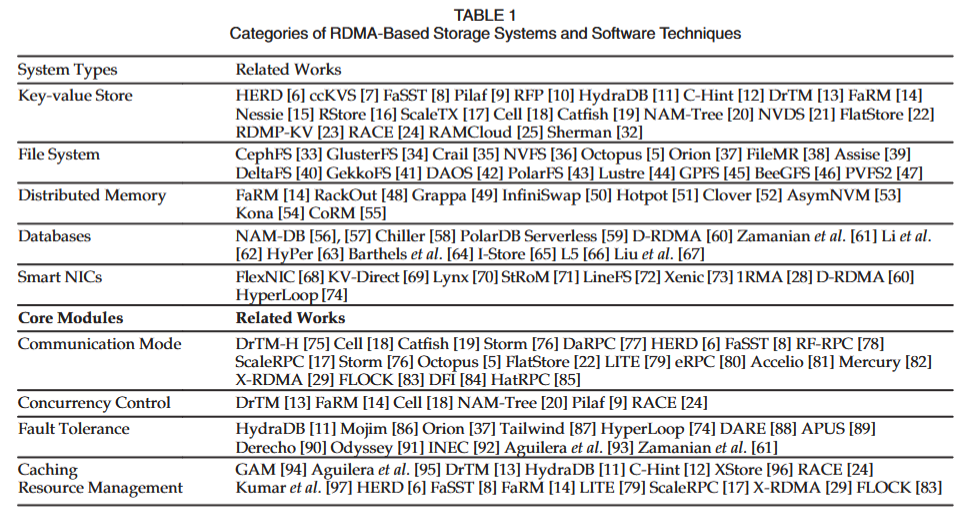
\includegraphics[width=0.5\textwidth]{Table_1_A_Survey_of_Storage_Systems_in_the_RDMA_Era}
\cite{Ma-PDS-2022}
%-----------------------------------------------------------------------------------------
%                       LOOSELY RELATED
%-----------------------------------------------------------------------------------------
%Loosely Related / Line of Work 
\section{Loosely Related but Evaluated}
    \subsection{CoRM: Compactable Remote Memory over RDMA}
    page based I think (re-read this)\cite{Taranov-ICMD-2021}

    \subsection{Rcmp: Reconstructing RDMA-Based Memory Disaggregation via CXL}
    page based and uses CXL, not comparable\cite{Wang-ACO-2024}
%-----------------------------------------------------------------------------------------


\bibliographystyle{acm}
\bibliography{relworks}
\end{document}